\section{Trade-off}
In this section a trade-off will be made between the previously listed video decoding frameworks, resulting into a conclusion in which a framework is chosen that will be used in the prototype application of this Bachelor project. In the trade-off, the following criteria are taken into consideration:
\begin{itemize}
	\item[-]Number of supported multimedia file formats.
	\item[-]Hardware decoding: to what degree does the framework support hardware accelerated decoding. 
	\item[-]Android version support.
	\item[-]Performance: framerate and image quality.
	\item[-]Updates: how often is the framework updated and maintained.
	\item[-]Documentation: quantity of documentation. 
	\item[-]Number of users.
\end{itemize}
In the following figure an overview of the trade-off is given which shows how each of the frameworks scored against each of the listed criteria.\\
\newline
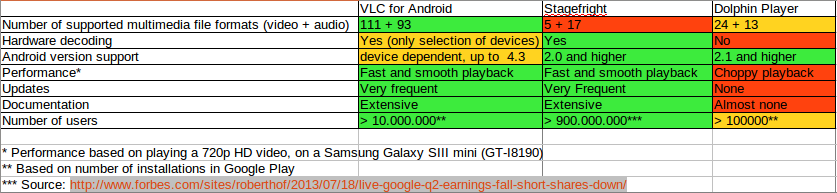
\includegraphics[width=350px]{video_decoding/tradeoff.png}\\
\newline
In the next figure, a cumulative view of the number of supported multimedia formats can be seen.\\
\newline
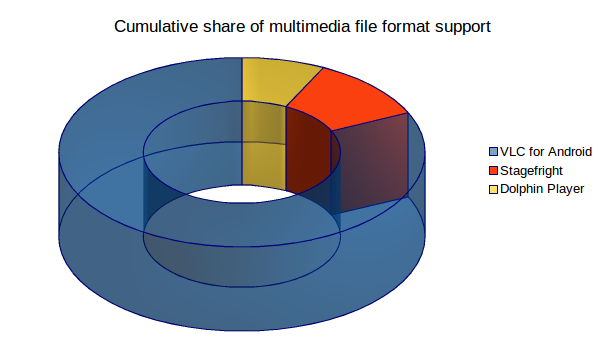
\includegraphics[width=250px]{video_decoding/cumulativeshare.png}\\
\newline
It should be noted that the supported file formats are overlapping. This means that Dolphin Player includes support for the all the file formats that are supported in Stagefright, plus an additional set of 22 file formats. VLC for Android supports all the file formats supported by the other frameworks, plus an additional set of 167 file formats.\\




